% Hands-on session: replicating Card and Krueger (1994) with AI assistants
% Compile: pdflatex ck_session.tex (twice). For facilitator notes on a second screen,
% uncomment the \setbeameroption line below.
\documentclass[aspectratio=169,11pt]{beamer}
\usetheme[progressbar=frametitle,numbering=fraction]{metropolis}
%\setbeameroption{show notes on second screen=right}

\usepackage{lmodern}
\usepackage[T1]{fontenc}
\input{glyphtounicode}
\pdfgentounicode=1
\usepackage{booktabs}
\usepackage{tikz}
\usepackage{fontawesome5}
\usepackage{amsmath}

\definecolor{ink}{HTML}{1B2A3A}
\definecolor{paper}{HTML}{F7F5EF}
\definecolor{accent}{HTML}{BC0031}% UvA red for all highlights
\definecolor{calm}{HTML}{2F6690}
\definecolor{soft}{HTML}{ECE8DD}
\setbeamercolor{normal text}{fg=ink,bg=paper}
\definecolor{uvared}{HTML}{BC0031}
\setbeamercolor{frametitle}{fg=white,bg=uvared}
\setbeamercolor{palette primary}{fg=paper,bg=ink}% standout slides stay navy
\setbeamercolor{frametitle}{fg=white,bg=uvared}
\setbeamercolor{background canvas}{bg=paper}
\setbeamercolor{progress bar}{fg=ink,bg=soft}
\setbeamercolor{alerted text}{fg=accent}
\setbeamercolor{block title}{fg=paper,bg=calm}
\setbeamercolor{block body}{fg=ink,bg=soft}
\setbeamercolor{block title alerted}{fg=paper,bg=accent}
\setbeamercolor{block body alerted}{fg=ink,bg=soft}

\urlstyle{same}
% Clickable links: a distinct link blue, underlined, so they read as links
\definecolor{linkblue}{HTML}{1A5FB4}
\definecolor{linklight}{HTML}{9CC4F0}
\hypersetup{colorlinks=true,urlcolor=linkblue,linkcolor=.}
\usepackage[normalem]{ulem}
\let\oldurl\url
\renewcommand{\url}[1]{{\color{linkblue}\uline{\oldurl{#1}}}}
\renewcommand{\ULthickness}{0.4pt}
\newcommand{\paperurl}{https://davidcard.berkeley.edu/papers/min-wage-ff-nj.pdf}
\newcommand{\dataurl}{https://davidcard.berkeley.edu/data_sets/njmin.zip}
% A prompt box meant to be copied from the PDF: no hyphenation, ragged right
\newcommand{\prompt}[2][\linewidth]{{\setlength{\fboxsep}{6pt}\colorbox{soft}{\parbox{\dimexpr#1-12pt}{\raggedright\hyphenpenalty=10000\exhyphenpenalty=10000\small #2}}}}
\newcommand{\copyhint}{{\scriptsize\color{calm}\faCopy[regular]\ copy and paste}}
\newcommand{\habit}[3]{\begin{minipage}[t]{0.47\textwidth}{\color{accent}\large #1}\hspace{0.5em}\textbf{#2}\\[0.1em]{\small #3}\end{minipage}}
\newcommand{\handson}[2]{\colorbox{accent}{\color{paper}\small\bfseries\faLaptopCode\ #1}\hspace{0.6em}{\small\color{accent}\bfseries #2}}

\title{Replicating a classic with AI assistants}
\subtitle{Card and Krueger (1994): minimum wages and fast-food employment}
\author{Joaquim Gromicho}
\institute{AI \& Research \textperiodcentered\ Lab 4, evening 3 \textperiodcentered\ 60 minutes, follow along in pairs}
\date{[date] \textperiodcentered\ [room]}
\setbeamerfont{subtitle}{size=\normalsize}
% UvA logo: full logo on the title slide, emblem in every frame title bar
\titlegraphic{\hfill\includegraphics[height=0.75cm]{figures/uva-logo.pdf}}
\addtobeamertemplate{frametitle}{}{%
\begin{tikzpicture}[remember picture,overlay]
\node[anchor=north east,inner sep=0pt] at (current page.north east) {\includegraphics[height=1.04cm]{figures/uva-emblem.jpg}};
\end{tikzpicture}}

\begin{document}

\maketitle
\note{Ask everyone to sit in pairs, one laptop per pair with Python and an AI assistant. The aim is not minimum-wage economics. The aim is learning to check research with an assistant: reproduce a published number, then find out which choices drive it.}

\begin{frame}{Plan}
\begin{tabular}{@{}p{0.13\textwidth}p{0.48\textwidth}p{0.3\textwidth}@{}}
\toprule
\textbf{Minutes} & \textbf{What happens} & \textbf{You do}\\
\midrule
0--5 & My area: optimization, and how I use agents & Listen\\
5--10 & The question, the paper, the design & Vote, then listen\\
10--30 & \alert{Round 1:} replicate Table 4 & Follow along, in pairs\\
30--42 & \alert{Round 2:} stress-test one choice & Pairs, one task each\\
42--47 & An assistant explains the paper & Watch and listen\\
47--60 & What no software settles & Discuss\\
\bottomrule
\end{tabular}\\[0.5em]
\small Homework: explain the paper to the public, and a one-page report.
\note{Two of six blocks are hands-on, and round 1 is a live demo that participants copy step by step. If time runs short, cut the explanation block, never the final discussion. Before the session: participants run get-data.ps1 and install the requirements from the lab4-replication folder, there is a hosted-notebook fallback, and the reference solution is ready but closed.}
\end{frame}

\section{My area: optimization}

\begin{frame}{How I work with agents}
\habit{\faBookOpen}{Read}{I ask for a slide deck that tells me a paper's main story.}\hfill
\habit{\faRedo}{Replicate}{Agents rebuild published results from the authors' data and code.}\\[1em]
\habit{\faVial}{Code and test}{Every number comes from a run, with checks that can fail.}\hfill
\habit{\faCodeBranch}{GitHub}{Version control and pull requests, also to open-source repositories.}\\[1em]
\habit{\faPen}{Write}{Agents draft articles, slides and emails; I rewrite them.}\hfill
\habit{\faBalanceScale}{Stay critical}{I question every iteration, and compare frontier models: Codex and Claude.}
\note{One minute. This deck itself is an example: Codex and Claude Code each replicated the paper independently, an agent made the maps, and the deck went to the course repository as a pull request.}
\end{frame}

\begin{frame}{What agents change for me}
\begin{alertblock}{Not more papers, but more ambitious ones}
Agents do not turn me into a paper mill. They let me take on research of a larger scope, especially where coding is a substantial part of the work.
\end{alertblock}
\vspace{1em}
\begin{alertblock}{A critical reviewer of the code}
I have written code by hand for thirty years, in many languages. That makes me very critical of how agents develop code: I read it, test it and push back.
\end{alertblock}
\note{One minute. The point to land: the gain is in scope and ambition, not in volume, and it depends on an experienced eye on the code.}
\end{frame}

\begin{frame}{Hands-On Mathematical Optimization with Python}
\small
A textbook with Krzysztof Postek, Alessandro Zocca and Jeffrey Kantor (Cambridge University Press, 2025). Every model is a notebook you can run, check and change: \url{https://mobook.github.io/MO-book/}\\[0.6em]
\textbf{Demo: an agent runs one of the book's notebooks} \copyhint\\[0.2em]
\prompt[\textwidth]{Run the notebook 02-production-planning-basic.ipynb and tell me the optimal plan and profit. Then: the demand for product U is capped at 40 units. What happens if that cap rises to 60? Change only that in a copy, run it, and show both results side by side.}\par
\vspace{0.8em}
\begin{columns}[T]
\begin{column}{0.44\textwidth}
\footnotesize
\begin{tabular}{@{}lrr@{}}
\toprule
& U $\le$ 40 & U $\le$ 60\\
\midrule
Profit & 2600 & 2600\\
Units of U, V & 20, 60 & 20, 60\\
Labour A, B used & 80, 100 & 80, 100\\
\bottomrule
\end{tabular}
\end{column}
\begin{column}{0.52\textwidth}
\footnotesize
\alert{Nothing changes.} The agent noticed the surprise and checked why: the cap on U was never binding; labour A and B are used up (shadow prices 70 and 50, the U cap 0).
\end{column}
\end{columns}
\note{About 90 seconds. Real run on 16 October 2026: a fresh agent in an empty folder with a copy of the book's notebook 01/02, about 2.3 minutes, no errors. It edited one line, model.y_U = pyo.Var(bounds=(0, 40)) to (0, 60), ran both notebooks, and checked the shadow prices with a small script of its own. Its comparison and log are in demo-notebook/. The point for the room: a what-if that changes nothing is still informative, and a good agent explains why instead of just reporting the numbers.}
\end{frame}

\begin{frame}{With agents: replicating a location benchmark}
\begin{columns}[c]
\begin{column}{0.52\textwidth}
\footnotesize
\textbf{The problem}\\
Brooklyn: choose 50 of 7,730 sites to cover as many of 2,504,700 people as possible within 800\,m.\\[0.4em]
\textbf{The published work}\\
Máximo, Cordeau and Nascimento (2025), with Java code.\\
{\scriptsize \url{https://doi.org/10.1111/itor.13387}\\ \url{https://github.com/vinymax10/AILS-MCLP}}\\[0.4em]
\textbf{What the agent did}\\
Compiled the authors' code, ran it for 60 seconds, checked the coverage.\\[0.4em]
\normalsize\alert{It recovered exactly the 50 published sites.}
\end{column}
\begin{column}{0.44\textwidth}
\centering
\includegraphics[height=0.62\textheight]{figures/kings_reference.png}\\
{\tiny Teal: covered \quad Orange: not covered \quad Diamonds: chosen sites}\\[0.3em]
{\scriptsize\color{accent}\bfseries The papers contain no maps of their solutions.\\ These maps are agentic work too.}
\end{column}
\end{columns}
\note{About 90 seconds. Maximal covering location problem, Kings County benchmark, ITOR 2025 (doi 10.1111/itor.13387). Codex (OpenAI) did the compiling, running and checking; an added harness recomputed the covered population from the selected sites and rejected a deliberately wrong objective. One unseeded 60-second trial, not a full replication. The papers show algorithm and performance figures but no maps of the solutions: Codex made these maps from the saved site sets, rescoring every solution on the same coverage graph. Builds on Fleur's historical notebooks and Parvathy's thesis work: check how they want to be credited.}
\end{frame}

\begin{frame}{We seemed to beat the literature}
\begin{columns}[c]
\begin{column}{0.56\textwidth}
\small
\begin{tabular}{@{}lr@{}}
\toprule
Solution & People covered\\
\midrule
Our Gurobi sites, our own scoring & \alert{2,024,813}\\
Published reference & 2,022,077\\
Authors' Java code, one run & 2,022,077\\
\midrule
Our Gurobi sites, scored their way & \alert{2,021,487}\\
\bottomrule
\end{tabular}\\[0.8em]
\normalsize
Our ``win'' came from a slightly different coverage rule: who counts as within 800\,m. Scored the same way, we cover 590 people \emph{fewer}.\\[0.6em]
\alert{Replication depends on the model's details, not only on the algorithm.}
\end{column}
\begin{column}{0.4\textwidth}
\centering
\includegraphics[height=0.68\textheight]{figures/kings_difference.png}\\[0.2em]
{\scriptsize Map made by the agent, not taken from the papers.}
\end{column}
\end{columns}
\note{About two minutes. The published value, the Java run and the rescoring all use the authors' coverage graph (779,676 site-person pairs). Our July Gurobi run used our own reconstruction; the distance conventions differ, for example the Java code rounds the angular distance to single precision before converting to metres. The map shows the few places where the two site sets cover different people. Gurobi stopped at its one-hour limit with a 0.16 percent gap, so nothing here is proven optimal, and run budgets differ, so no runtime comparison. Same lesson as the footnote we will find in Card and Krueger.}
\end{frame}

\begin{frame}[standout]
Optimization or econometrics:\\
the agent gives you a number in minutes.\\[1em]
\normalsize Knowing why it is right is still your job.\\[0.6em]
Let's try that together, on a famous paper.\\[1.2em]
\scriptsize A longer example with agents: {\colorlet{linkblue}{linklight}\hypersetup{urlcolor=linklight}\url{https://github.com/gromicho/OceanCleanupDataChallenge}}
\note{30 seconds. Transition to the hands-on part. The Ocean Cleanup repository is there for anyone who wants a full end-to-end example.}
\end{frame}

\begin{frame}[standout]
\faHandPaper[regular]\ Vote with your hand\\[1em]
\normalsize New Jersey raises the minimum wage from \$4.25 to \$5.05.\\
Pennsylvania, next door, does not.\\
What happens to fast-food employment, relative to Pennsylvania?\\[1em]
\large A.\ it falls \quad B.\ no change \quad C.\ it rises
\note{Count hands and write the split on the board. Come back to it at the end: did the evidence move anyone, and should it have?}
\end{frame}

\section{The paper}

\begin{frame}{A natural experiment}
\begin{itemize}
\item 1 April 1992: New Jersey's minimum wage rises from \$4.25 to \$5.05.
\item Pennsylvania, next door, keeps \$4.25: the comparison group.
\item Telephone survey of 410 fast-food restaurants: Burger King, KFC, Roy Rogers, Wendy's.
\item Wave 1 in February--March 1992, wave 2 seven to eight months later.
\end{itemize}
\vspace{0.6em}
\begin{block}{Everything is public}
\small
\faFilePdf\ Paper: \url{\paperurl}\\[0.2em]
\faDatabase\ Data, codebook and the authors' SAS program: \url{\dataurl}\\[0.3em]
\footnotesize SAS is commercial statistics software, standard in 1990s economics. You do not need it: the agent reads \texttt{check.sas} and rewrites it in Python.
\end{block}
\note{Point out that the data and the original program are public. That is what makes this paper a good exercise: students can rebuild every number and question every choice.}
\end{frame}

\begin{frame}{Difference in differences}
\begin{columns}[c]
\begin{column}{0.5\textwidth}
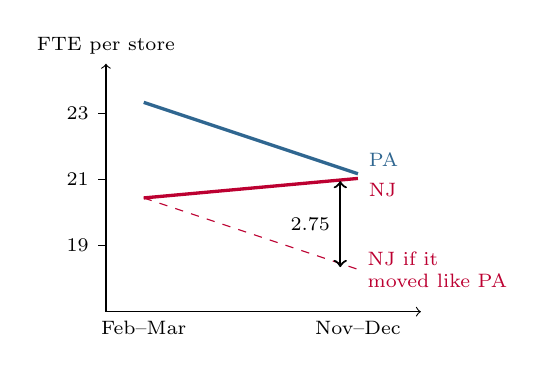
\begin{tikzpicture}[x=3.2cm,y=0.42cm]
\draw[->] (0,17) -- (1.25,17);
\draw[->] (0,17) -- (0,24.5) node[above,font=\scriptsize] {FTE per store};
\foreach \y in {19,21,23} \draw (0,\y) -- (-0.03,\y) node[left,font=\scriptsize] {\y};
\node[below,font=\scriptsize] at (0.15,17) {Feb--Mar};
\node[below,font=\scriptsize] at (1,17) {Nov--Dec};
\draw[calm,very thick] (0.15,23.33) -- (1,21.17) node[right,yshift=5pt,font=\scriptsize] {PA};
\draw[accent,very thick] (0.15,20.44) -- (1,21.03) node[right,yshift=-4pt,font=\scriptsize] {NJ};
\draw[accent,dashed] (0.15,20.44) -- (1,18.28) node[right,font=\scriptsize,align=left] {NJ if it\\moved like PA};
\draw[<->,thick] (0.93,18.35) -- (0.93,20.95) node[midway,left,font=\scriptsize] {2.75};
\end{tikzpicture}
\end{column}
\begin{column}{0.45\textwidth}
\begin{tabular}{@{}lrrr@{}}
\toprule
& Before & After & Change\\
\midrule
PA & 23.33 & 21.17 & $-2.16$\\
NJ & 20.44 & 21.03 & $+0.59$\\
\midrule
\multicolumn{3}{@{}l}{Difference in changes} & \alert{$+2.75$}\\
\bottomrule
\end{tabular}\\[0.6em]
\footnotesize FTE: full-time equivalent, part-timers count half.\\
Our computation; the paper prints 2.76.
\end{column}
\end{columns}
\note{The dashed line is the assumption that does all the work: without the wage rise, New Jersey would have moved like Pennsylvania. Keep this in mind for the final discussion.}
\end{frame}

\begin{frame}{The regressions in Table 4}
\small
\[
\Delta E_i = a + b\,X_i + c\,\mathit{NJ}_i + \varepsilon_i
\qquad\text{or}\qquad
\Delta E_i = a' + b'X_i + c'\,\mathit{GAP}_i + \varepsilon'_i
\]
\begin{itemize}
\item $\Delta E_i$: change in FTE employment at store $i$.
\item $X_i$: chain and company-ownership dummies; in model (v) also region dummies.
\item $\mathit{GAP}_i$: proportional wage rise store $i$ needs to reach \$5.05; zero in Pennsylvania and for New Jersey stores already at \$5.05.
\end{itemize}
\begin{center}
\begin{tabular}{@{}lccccc@{}}
\toprule
Published & (i) & (ii) & (iii) & (iv) & (v)\\
\midrule
NJ dummy & 2.33 (1.19) & 2.30 (1.20) & & & \\
GAP & & & 15.65 (6.08) & 14.92 (6.21) & 11.91 (7.39)\\
\bottomrule
\end{tabular}\\[0.3em]
\footnotesize 357 stores. This is your target.
\end{center}
\note{GAP uses variation inside New Jersey as well as between the states. Leave the table on screen during round 1.}
\end{frame}

\section{Hands-on}

\begin{frame}{Round 1: replicate Table 4}
\handson{20 minutes}{follow along: I type it, you type it}\\[0.6em]
\textbf{1. Replicate} \copyhint\\[0.2em]
\prompt{Download into this folder \url{\paperurl}\newline and \url{\dataurl} and unzip it.\newline Read Table 4 in the paper. Translate check.sas into Python with pandas and NumPy, reproduce Table 4, and print each coefficient and standard error next to the value in the paper.}\\[0.1em]
{\scriptsize Claude Code asks before it downloads: allow it. Download blocked? Save both files in the folder yourself.}\\[0.5em]
\textbf{2. Then ask} \copyhint\\[0.2em]
\prompt{Which stores were left out of the regressions, and why?}\\[0.4em]
\footnotesize\textbf{Done when:} \alert{357} stores, all \alert{five} coefficients and standard errors match. \quad \textbf{You need:} Claude Code (Pro), Python with pandas and NumPy, an empty folder.
\note{Walk around. Common traps: missing values read as zero; closed stores dropped instead of kept with zero employment; GAP computed for Pennsylvania. Pairs that finish early start the follow-up question. Reference: a full run takes about two seconds. The paper is a scanned PDF: fetching it as a web page returns no readable text, but Claude Code reads the saved PDF's pages as images, which is why the prompt downloads it first (tested 15 October 2026).}
\end{frame}

\begin{frame}[fragile]{Checkpoint: what the agent returned}
\textbf{Hands up:} all five match? \quad three or four? \quad still debugging?\\[0.4em]
{\footnotesize A fresh agent, given only the Round 1 prompt. Lines copied from its output.}
\begin{beamercolorbox}[sep=4pt]{block body}
\fontsize{6.4}{7.4}\selectfont
\begin{verbatim}
Stores in public.dat: 410; in DATA C1 subset: 357; used in PROC REG (no missing in any model var): 357  [paper: 357]

Col   Regressor      Coef   Paper      SE   Paper    SER  Paper  p(ctrl)  Paper
(i)   NJ             2.33    2.33    1.19    1.19   8.79   8.79        -      -
(ii)  NJ             2.30    2.30    1.20    1.20   8.78   8.78     0.34   0.34
(iii) GAP           15.65   15.65    6.08    6.08   8.76   8.76        -      -
(iv)  GAP           14.92   14.92    6.21    6.21   8.76   8.76     0.44   0.44
(v)   GAP           11.91   11.91    7.39    7.39   8.74   8.75     0.31   0.40
(v)*  GAP           11.98   11.91    7.42    7.39   8.75   8.75     0.40   0.40
\end{verbatim}
\end{beamercolorbox}
\vspace{0.3em}
\small\textbf{Tell the room:} what did your assistant get wrong first? Did it, too, flag column (v)?\\
{\footnotesize\color{accent}\bfseries Unasked, the agent flagged column (v); its line (v)* adds ownership.}
\note{Collect two or three stories. The output is verbatim from a fresh agent run on 15 October 2026 (a Claude Code subagent with no access to our earlier work, working in an empty folder; it was told where Python is installed and that Table 4 is on page 10 of the PDF). It downloaded the files, read Table 4 from the rendered page, translated check.sas, and no command failed. It found 357 stores and printed the extra (v)* line on its own. Its log and script are in demo-run/. Its only other difference: mean change -0.238 against the paper's -0.237, a rounding difference. Pairs that are stuck get the reference script now, so everyone can do round 2.}
\end{frame}

\begin{frame}{Dry run: 2.6 minutes, step by step}
\centering
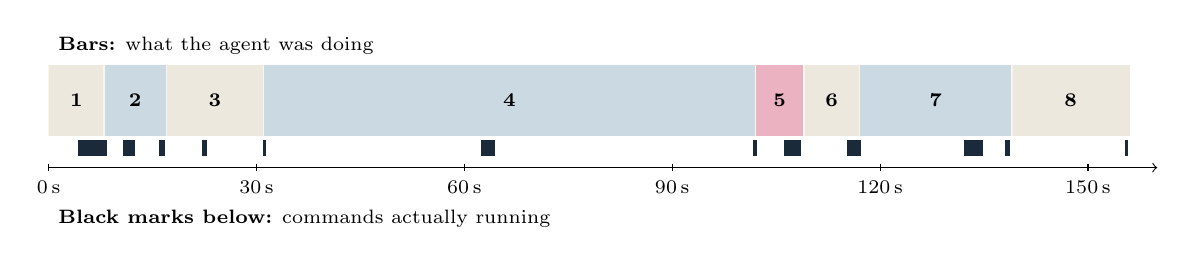
\begin{tikzpicture}[x=0.088cm,y=1cm,font=\scriptsize]
% phases: start, end, number
\foreach \a/\b/\n/\c in {0/8/1/soft,8/17/2/calm!25,17/31/3/soft,31/102/4/calm!25,102/109/5/accent!30,109/117/6/soft,117/139/7/calm!25,139/156/8/soft}{
  \fill[\c] (\a,0) rectangle (\b,0.9);
  \draw[paper,line width=0.6pt] (\a,0) -- (\a,0.9);
  \node at ({(\a+\b)/2},0.45) {\bfseries\n};
}
% command execution intervals (seconds), from the transcript
\foreach \a/\b in {4.3/8.4,10.8/12.5,15.9/16.8,22.2/22.8,30.9/31.4,62.4/64.4,101.7/102.2,106.1/108.6,115.2/117.3,132.1/134.8,138.0/138.7,155.4/155.8}{
  \fill[ink] (\a,-0.25) rectangle (\b,-0.05);
}
\draw[->] (0,-0.4) -- (160,-0.4);
\foreach \t in {0,30,60,90,120,150} {\draw (\t,-0.35) -- (\t,-0.45) node[below] {\t\,s};}
\node[anchor=west] at (0,1.15) {\textbf{Bars:} what the agent was doing};
\node[anchor=west] at (0,-1.05) {\textbf{Black marks below:} commands actually running};
\end{tikzpicture}\\[0.5em]
\footnotesize
\begin{tabular}{@{}rlrl@{}}
1 & Download paper and data & 5 & \alert{First run: all values match}, (v) flagged\\
2 & Unzip; read code, codebook, Table 4 & 6 & Follow-up: which stores were dropped\\
3 & Check the data layout; start a log & 7 & Save output and log\\
4 & \alert{Write the Python translation (71 s)} & 8 & Write its report\\
\end{tabular}
\note{Times from the timestamps in the agent's transcript, 15 October 2026, measured from the moment it received the prompt; total 155.8 seconds. One run, so a description, not a benchmark.}
\end{frame}

\begin{frame}[fragile]{What the agent wrote: SAS into Python}
\fontsize{6.6}{7.8}\selectfont
\begin{columns}[T]
\begin{column}{0.36\textwidth}
\textbf{\normalsize check.sas (1997)}
\end{column}
\begin{column}{0.6\textwidth}
\textbf{\normalsize replicate\_table4.py (the agent)}
\end{column}
\end{columns}
\vspace{0.2em}
\begin{columns}[T]
\begin{column}{0.36\textwidth}
\begin{beamercolorbox}[sep=3pt]{block body}
\begin{verbatim}
EMPTOT=EMPPT*.5 + EMPFT + NMGRS;
\end{verbatim}
\end{beamercolorbox}
\end{column}
\begin{column}{0.6\textwidth}
\begin{beamercolorbox}[sep=3pt]{block body}
\begin{verbatim}
d["emptot"] = d.emppt * 0.5 + d.empft + d.nmgrs
\end{verbatim}
\end{beamercolorbox}
\end{column}
\end{columns}
\vspace{0.2em}
\begin{columns}[T]
\begin{column}{0.36\textwidth}
\begin{beamercolorbox}[sep=3pt]{block body}
\begin{verbatim}
DATA C1;
SET CHECK;
IF DEMP NE . ;
IF CLOSED=1 OR (CLOSED=0 AND DWAGE NE .);
\end{verbatim}
\end{beamercolorbox}
\end{column}
\begin{column}{0.6\textwidth}
\begin{beamercolorbox}[sep=3pt]{block body}
\begin{verbatim}
# DATA C1: IF DEMP NE .; IF CLOSED=1 OR (CLOSED=0 AND DWAGE NE .);
c1 = d[d.demp.notna()]
c1 = c1[(c1.closed == 1) | ((c1.closed == 0) & c1.dwage.notna())]
\end{verbatim}
\end{beamercolorbox}
\end{column}
\end{columns}
\vspace{0.2em}
\begin{columns}[T]
\begin{column}{0.36\textwidth}
\begin{beamercolorbox}[sep=3pt]{block body}
\begin{verbatim}
MODEL DEMP=GAP BK KFC ROYS
  CENTRALJ SOUTHJ PA1 PA2;
\end{verbatim}
\end{beamercolorbox}
\end{column}
\begin{column}{0.6\textwidth}
\begin{beamercolorbox}[sep=3pt]{block body}
\begin{verbatim}
"gap+chain+region": ["gap", "bk", "kfc", "roys", "centralj",
                     "southj", "pa1", "pa2"],
# Variant: column (v) as the paper's notes describe it
VARIANT = ["gap", "bk", "kfc", "roys", "co_owned", ...]
\end{verbatim}
\end{beamercolorbox}
\end{column}
\end{columns}
\vspace{0.6em}
{\footnotesize
\textbf{Look closer:} the paper's values are \alert{typed in} from the PDF image; matches are \alert{checked by eye}, nothing fails on a mismatch; and to obey ``pandas and NumPy'' it \alert{hand-coded} the F-test p-value (30 lines).}
\note{All code lines are copied from check.sas and from demo-run/replicate_table4.py; the SAS MODEL statement is wrapped onto two lines here and the VARIANT list is shortened with "...". Point out how literal the translation is: the SAS line is even kept as a comment. Then the three cautions: a misread digit in the typed-in paper values would silently become the target; a printed side-by-side table cannot fail; and the literal prompt produced extra code nobody asked for (scipy was installed).}
\end{frame}

\begin{frame}{Dry run: where the time went}
\begin{columns}[c]
\begin{column}{0.5\textwidth}
\centering
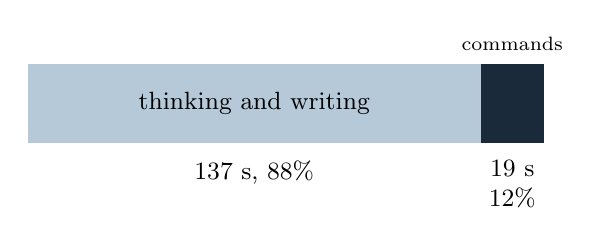
\begin{tikzpicture}[x=0.042cm,font=\small]
\fill[calm!35] (0,0) rectangle (137,1);
\fill[ink] (137,0) rectangle (156,1);
\node at (68.5,0.5) {thinking and writing};
\node[anchor=north] at (68.5,-0.1) {137 s, 88\%};
\node[anchor=north,align=center] at (146.5,-0.1) {19 s\\12\%};
\node[anchor=south,align=center,font=\scriptsize] at (146.5,1.05) {commands};
\end{tikzpicture}
\end{column}
\begin{column}{0.46\textwidth}
\begin{itemize}
\item Downloading, unzipping and running the code took seconds.
\item Almost all the time is the agent \alert{reading, reasoning and writing}; nearly half of it on the script.
\item The first run matched; nothing had to be fixed.
\end{itemize}
\end{column}
\end{columns}
\vspace{1em}
\begin{alertblock}{Expect longer in the room}
Claude Code asks permission before downloads and commands, Python has to be found, and models and speeds differ. Round 1 has 20 minutes for that reason.
\end{alertblock}
\note{Command time is the sum of the tool-execution intervals in the transcript (18.7 s); the rest is model time. The run was a subagent told where Python is installed and on which PDF page Table 4 is, so a participant's first run will be slower.}
\end{frame}

\begin{frame}{Round 2: stress-test one choice}
\handson{12 minutes}{one letter per pair; report one number and one sentence}\hfill\copyhint\\[0.5em]
\begin{tabular}{@{}l@{\hspace{0.6em}}l@{}}
\textbf{A} & \prompt[0.9\textwidth]{Re-run model (i) on all 384 stores with employment data. Which stores does Table 4 leave out, and how did their employment change?}\\[0.35em]
\textbf{B} & \prompt[0.9\textwidth]{Re-run all five models with robust (HC1) standard errors. Is the New Jersey effect still significant at 5\%?}\\[0.35em]
\textbf{C} & \prompt[0.9\textwidth]{Re-run models (i) and (iii) counting part-time workers as 0, 0.4, 0.6 and 1 instead of 0.5.}\\[0.35em]
\textbf{D} & \prompt[0.9\textwidth]{Re-run model (i) without the six closed stores. Then set the four temporarily closed stores to zero instead.}\\[0.35em]
\textbf{E} & \prompt[0.9\textwidth]{Add company ownership to model (v), as the Table 4 footnote says. Compare with the code.}\\
\end{tabular}
\note{Assign letters A to E around the room. With more than five pairs, give each letter to two pairs: they compare before reporting, which gives each a second opinion.}
\end{frame}

\begin{frame}{Round 2, advanced cards: the econometrics behind Table 5}
\handson{optional}{for pairs who finish early, or as homework}\hfill\copyhint\\[0.6em]
\begin{tabular}{@{}l@{\hspace{0.6em}}l@{}}
\textbf{F} & \prompt[0.9\textwidth]{Is a model in changes right? Add wave-1 employment to model (iv) and instrument it with the number of cash registers (NREGS) and registers open at 11:00 (NREGS11). Compare with plain OLS.}\\[0.5em]
\textbf{G} & \prompt[0.9\textwidth]{Reproduce Table 5 of the paper, rows 1 to 9 and 12. Print each value next to the paper's, and say which cells you cannot match and why.}\\
\end{tabular}\\[0.8em]
\small \textbf{F} is an instrumental-variables test from the paper's text (p.\,784). \textbf{G} is a partial replication: some rows are defined only vaguely in the paper.
\note{F: measurement error in wave-1 employment makes plain OLS of the change on the level mechanically negative; the registers are instruments for the true store size. G: rows 10 and 11 need ZIP codes, which the public file lacks, so they are left out on purpose.}
\end{frame}

\begin{frame}{Round 2: what we found}
\begin{tabular}{@{}lp{0.72\textwidth}@{}}
\toprule
\textbf{A} Sample & 384 $\to$ 357 moves the NJ estimate from 2.75 to 2.33. The 27 dropped stores \emph{work against} the finding: 19 NJ stores gained 4.55 FTE, 8 PA stores lost 3.59.\\
\textbf{B} Standard errors & NJ dummy: conventional 1.19 ($t\approx1.96$), robust 1.45 ($t\approx1.61$).\\
\textbf{C} Part-timers & Weight 0 to 1: NJ from 2.55 to 2.10; GAP from 18.16 to 13.15.\\
\textbf{D} Closures & Drop the six: 2.28 (1.19). Temporary closures as zero: 2.51 (1.18), 388 stores.\\
\textbf{E} Footnote vs code & Code 11.91 (7.39); with ownership 11.98 (7.42). And there is more: see the next slide.\\
\bottomrule
\end{tabular}\\[0.6em]
\small Compare with the board first. Our reference run, one machine, one tool.
\note{Ask each pair to read their number before revealing this slide. Discuss which choice moves the estimate most, and which one changes the conclusion (B: significance depends on the formula). Also: in proportional terms the effect is 5.2 percent with a standard error of 5.1 percent, which the paper itself reports.}
\end{frame}

\begin{frame}{Why replicate: one footnote, two regressions}
\begin{columns}[T]
\begin{column}{0.31\textwidth}
\begin{block}{The paper says}
\small Footnote b of Table 4: model (v) includes the chain dummies \emph{and} company ownership.
\end{block}
\end{column}
\begin{column}{0.31\textwidth}
\begin{block}{The code does}
\small \texttt{check.sas} runs model (v) with the chain and region dummies, \emph{without} ownership.
\end{block}
\end{column}
\begin{column}{0.31\textwidth}
\begin{block}{The table shows}
\small Coefficient 11.91 (7.39): the code's regression.\\[0.2em]
SER 8.75 and $p=0.40$: the footnote's regression.
\end{block}
\end{column}
\end{columns}
\vspace{1em}
\begin{alertblock}{The point}
Reading the paper, you would never notice. Only rebuilding every number shows that one column mixes two regressions. Small here, but this is how you learn what a paper actually did.
\end{alertblock}
\note{Two minutes, right after the Round 2 results. Our run: without ownership 11.913 (7.394), SER 8.740, p = 0.308; with ownership 11.979 (7.419), SER 8.753, p = 0.405. Columns (ii) and (iv) reproduce completely, including their p-values, so the method is not the issue. That the table was assembled from two runs is our inference; the paper and code cannot confirm it. It changes no conclusion.}
\end{frame}

\begin{frame}{Advanced cards: what we found}
\begin{columns}[T]
\begin{column}{0.47\textwidth}
\textbf{F: instrumental variables}\\[0.3em]
\small
\begin{tabular}{@{}lr@{}}
\toprule
Coefficient of wave-1 FTE & \\
\midrule
Paper, IV & 0.04 (0.24)\\
Ours, IV (348 stores) & 0.03 (0.23)\\
Ours, plain OLS & \alert{$-0.56$ (0.04)}\\
\bottomrule
\end{tabular}\\[0.4em]
Plain OLS is pulled down by measurement error; the instrument removes that. A model in changes is fine.
\end{column}
\begin{column}{0.49\textwidth}
\textbf{G: Table 5}\\[0.3em]
\small
\alert{21 of 36} published cells match at two decimals.\\[0.3em]
\footnotesize
\textbf{Match:} weighting by initial size, the Pennsylvania placebo, most call-back and closure rows.\\[0.2em]
\textbf{No match:} interview-week dummies; percentage columns of the FTE variants.\\[0.2em]
\textbf{Paper vs paper:} Table 5 prints 2.30 (1.19) where Table 4 prints 2.30 (1.20).
\end{column}
\end{columns}
\vspace{0.6em}
\begin{alertblock}{The pattern}
Robustness checks with a clear definition reproduce; the vaguely described ones do not.
\end{alertblock}
\note{Our run, 16 October 2026, advanced/ck_table5_iv.py. F: the paper reports only the IV coefficient; the OLS line is ours. Nine stores lack register counts, which may explain the 0.01 difference. G: rows 3-5 change columns match once the sample is held at 357 stores; dividing by wave-1 instead of average employment brings the percentage columns close (0.27 vs 0.28, 0.32 vs 0.30, 0.20 vs 0.17) but not exact. Row 6 excludes 31 shore stores where the paper says 35; row 8 excludes 63 stores where the paper says 70. Rows 10-11 need ZIP codes.}
\end{frame}

\begin{frame}{An assistant explains the paper}
\begin{columns}[T]
\begin{column}{0.4\textwidth}
With the replication done, the same assistant wrote three explanations for the public:
\begin{itemize}
\item an eight-slide deck
\item a 600-word newspaper article
\item a podcast, here cut to one minute
\end{itemize}
\vspace{0.3em}
\alert{Listen for:} what does it simplify, and is that still true?
\end{column}
\begin{column}{0.55\textwidth}
\includegraphics[page=4,width=0.48\linewidth]{ck_explainer.pdf}\hfill
\includegraphics[page=7,width=0.48\linewidth]{ck_explainer.pdf}\\[0.3em]
\scriptsize Two slides of the example deck. ``Why it mattered'' relies on the assistant's background knowledge, not on the paper: it needs checking.
\end{column}
\end{columns}
\note{Five minutes. Play ck_podcast_1min.mp3 (one minute). Then show the two slides and ask: which claim would you check first? Mention that the article and the full podcast script are in the course folder. Making their own version is homework.}
\end{frame}

\section{Discussion}

\begin{frame}[standout]
Only two states.\\[0.8em]
\normalsize Any shock that hits New Jersey but not Pennsylvania\\
looks exactly like a minimum-wage effect.\\[1em]
\large What evidence would convince you?
\note{Think, pair, share: one minute alone, two in pairs, then collect answers. Expect: more states or more episodes, pre-trends, a placebo group such as high-wage NJ stores (the paper uses this), other outcomes like prices. Point out that no standard-error formula fixes this: it is a design question. Return to the opening vote.}
\end{frame}

\begin{frame}{Homework: explain it to the public}
\textcolor{accent}{\small\bfseries Pick one format. Paste its prompt into the assistant that holds your replication.} \copyhint\par\medskip
\begin{columns}[T]
\begin{column}{0.32\textwidth}
\textbf{Slide deck}\\[0.2em]
\prompt{Using the paper and our results, write an HTML slide deck of at most eight slides explaining this study to first-year students. Say where each number comes from.}
\end{column}
\begin{column}{0.32\textwidth}
\textbf{Newspaper article}\\[0.2em]
\prompt{Using the paper and our results, write a 600-word newspaper article about this study. Invent no quotes. Include what it cannot show.}
\end{column}
\begin{column}{0.32\textwidth}
\textbf{Podcast script}\\[0.2em]
\prompt{Using the paper and our results, write a five-minute podcast script for a host and an economist. End with the problem of having only two states.}
\end{column}
\end{columns}
\vspace{0.5em}
\textbf{\small Optional, to hear the podcast:}\\[0.2em]
\prompt[\textwidth]{Turn the script into one audio file with two of my computer's built-in voices. Install nothing.}
\note{Homework. Assign formats so all three appear in the group. Participants bring their fact-check to the next session or post it in the forum. Audio option: Windows has built-in voices (System.Speech, e.g. Zira and David) and macOS has the say command, so no install is needed; on Linux a voice such as espeak usually has to be installed. Our one-minute example (ck_podcast_1min.mp3) was made this way on Windows; it sounds clearly synthetic. Online voice services sound better but send the script to an outside service.}
\end{frame}

\begin{frame}{Homework: fact-check it, and report}
\begin{columns}[T]
\begin{column}{0.5\textwidth}
\textbf{Fact-check your explanation}
\begin{enumerate}
\item Does every number appear in the paper or in your results?
\item Which sentence claims more than the study shows?
\item What important limit is missing?
\item Is any quote, source or name invented?
\end{enumerate}
\end{column}
\begin{column}{0.45\textwidth}
\textbf{One-page report}
\begin{itemize}
\item your prompts, in order
\item the modelling choices you made or accepted
\item your checks, and how they could have failed
\item what you still do not trust
\end{itemize}
\end{column}
\end{columns}
\vspace{0.6em}
\begin{alertblock}{Exit question, tonight}
Which single choice would you report first in a referee report on this paper, and why?
\end{alertblock}
\note{Deadline and template: [link]. Collect the exit question before people leave.}
\end{frame}

\begin{frame}{Take-aways}
\begin{itemize}
\item An assistant reproduces the published numbers in minutes; \alert{knowing why they are right} takes the rest of the session.
\item The useful findings are in the \alert{choices}: sample, errors, weights, closures, code vs footnote.
\item Ask a \alert{second} tool or person; disagreement is information.
\item An assistant writes a fluent explanation in minutes; \alert{every number and claim} in it still needs checking.
\item Reproduction is not causal proof: the \alert{design} carries the argument.
\end{itemize}
\vspace{0.8em}
\footnotesize
\faFilePdf\ Paper: \url{\paperurl}\\
\faDatabase\ Data and program: \url{\dataurl}
\note{Close by asking whether the vote from the start would change now.}
\end{frame}

\begin{frame}{Not yet tested}
\begin{alertblock}{The podcast as audio on a Mac}
We have not tested whether the optional audio prompt produces a two-voice file on a Mac.\\[0.4em]
On Windows we did it ourselves for the one-minute version, with the built-in voices. Joining two voices into one file is easy on Windows. On a Mac it may take Claude Code a little more work.
\end{alertblock}
\vspace{0.6em}
\small If you try it on a Mac, please tell us how it went.
\note{An honest last slide: what this preparation did not check. The one-minute example is ck_podcast_1min.mp3, made with the Windows voices Zira and David.}
\end{frame}


\end{document}
